\section{Digitální signálové procesy}
-Digitální signálové procesy, základní architektury, systém zpracování instrukcí (CISC,
RISK, VLIW, CLIW), nástroje k dosažení vysokého výkonu DSP procesorů. ARM
architektura, charakteristika a základní vlastnosti.

\subsection{DSP}
Digitální signálový procesor nebo také digitální signální procesor (zkratka DSP) je mikroprocesor, jehož návrh je optimalizován pro algoritmy používané při zpracování digitálně reprezentovaných signálů. Hlavním nárokem na systém bývá průběžné zpracování velkého množství dat „protékajících“ procesorem.

Jedním ze základních důvodů k vytvoření DSP byl fakt, že klasické analogové obvody sloužící pro zpracování signálu bývají náročné z hlediska návrhu, nastavení, provedení a reprodukovatelnosti, přičemž jakmile jsou vyrobeny, nelze jejich funkci téměř modifikovat. Ve srovnání s tím cena „digitálního“ křemíku stále klesá a výkon roste.

 Analogový signál je nejprve převeden A/D převodníkem na digitální a v této podobě je průběžně zpracováván digitálním signálovým procesorem. Zpracovaný digitální signál je D/A převodníkem zpět převeden na analogový. V mnoha zařízeních prochází signál tímto řetězcem v reálném čase, ale na některých signálech je potřeba provést tak složité a výpočetně náročné algoritmy, že to ani velmi rychlý DSP procesor v reálném čase nestihne a digitalizovaná data musí být nejprve zaznamenána do paměti a odtamtud teprve postupně zpracovávána.
    \begin{figure}[h]
   \begin{center}
     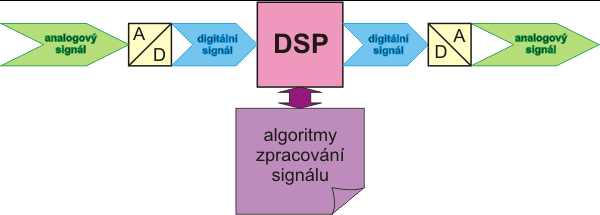
\includegraphics[scale=0.4]{images/DSP.png}
   \end{center}
   \caption{Digitální signálový procesor}
  \end{figure} 
 
 Typický digitální signálový procesor je vystavěn na harvardské architektuře. Tato architektura má oproti von Neumannovu modelu počítače oddělenou paměť pro program od paměti pro data. V praxi to znamená, že data a kód programu využívají vlastní sběrnice, což zvyšuje propustnost systému.
 
Základním dělením digitálních signálových procesorů je dělení podle použité aritmetiky. Existují DSP pracující:\\
v celočíselné aritmetice\\
v aritmetice s pevnou řádovou čárkou\\
v aritmetice s plovoucí řádovou čárkou\\

\textbf{Procesory s celočíselnou aritmetikou} jsou sice levné, ale algoritmy výpočtů stále narážejí na nutnost převádět reálná čísla na celá a mezivýsledky výpočtů se musí neustále upravovat tzv. normalizacemi. Proto je vývoj algoritmů v těchto typech procesorů výrazně náročnější. Hodí se proto zejména pro masovou produkci výrobků, kde nevadí poněkud vyšší cena vývoje, ale důležitá je zejména cena samotné součástky.

\textbf{Procesory s plovoucí řádovou čárkou} jsou sice složitější a dražší, ale vývoj softwaru je pro ně výrazně jednodušší. Nevýhodou zde může být rovněž vyšší spotřeba energie.

\textbf{Procesory s pevnou řádovou čárkou} mohou sice být určitým kompromisem, ale prakticky je nelze jasně odlišit od procesorů pracujících v celočíselné aritmetice.

Dalším kritériem pro dělení digitálních signálových procesorů je šířka jejich datové sběrnice. Ta bývá od 16 bitů výše. Další dělení může být na jednojádrové nebo vícejádrové DSP. 

\subsection{Nástroje k dosažení vysokého výkonu DSP procesorů}
Zrychlení výpočtů se dosahuje pomocí specializovaných výpočetních jednotek procesoru, které dokážou pracovat paralelně. Typický DSP má kromě aritmeticko-logické jednotky (ALU) navíc rychlou násobičku, která dokáže operaci násobení s přičítáním A ← A + B.k. Tato operace je základní operací většiny algoritmů digitálního zpracování signálu. DSP zpravidla obsahuje dvě nebo více nezávislých adresních jednotek, tzv. DAG (Data Address Generator), adresujících data v lineárních nebo kruhových bufferech. Typický DSP tak umožňuje během jednoho taktu provést jeden krok skalárního násobení dvou vektorů (vynásobení hodnot ze dvou bufferů, přičtení do akumulátoru, posun na další index v bufferech). Procesor s klasickou architekturou by na stejnou operaci potřeboval několik taktů (např. 1. načtení hodnoty z prvního bufferu, 2. vynásobení hodnotou z druhého bufferu, 3. přičtení výsledku do akumulátoru, 4. posun adresy prvního bufferu, 5. posun adresy druhého bufferu).

Oproti univerzálním procesorům mohou (ale nemusí) být v DSP zjednodušeny některé funkce, například nemusí být možné adresovat paměť po bajtech. Taková zjednodušení mohou vést k problémům s přenositelností kódu psaného ve vyšších programovacích jazycích, nebo k větší spotřebě paměti a strojového času při jiných úlohách, než je zpracování signálu.
 
\subsection{Základní architektury}
\subsubsection{Von Neumannova architektura}
Číslicový počítač (ČP) se skládá z následujících funkčních
jednotek:
\begin{itemize}
\item paměť (vnitřní, operační paměť), řadič,
\item aritmetická a logická jednotka (ALJ),
\item vstupní a výstupní jednotky.
\end{itemize}
2) Struktura číslicového počítače není závislá na typu řešené
úlohy, je univerzální, číslicový počítač se programuje
obsahem operační paměti.\\
3) Instrukce programu i operandy, s nimiž program pracuje,
jsou uloženy v téže paměti (operační paměti), jde-li o
instrukci či o operand rozpoznává počítač „z kontextu“.\\
    \begin{figure}[h]
   \begin{center}
     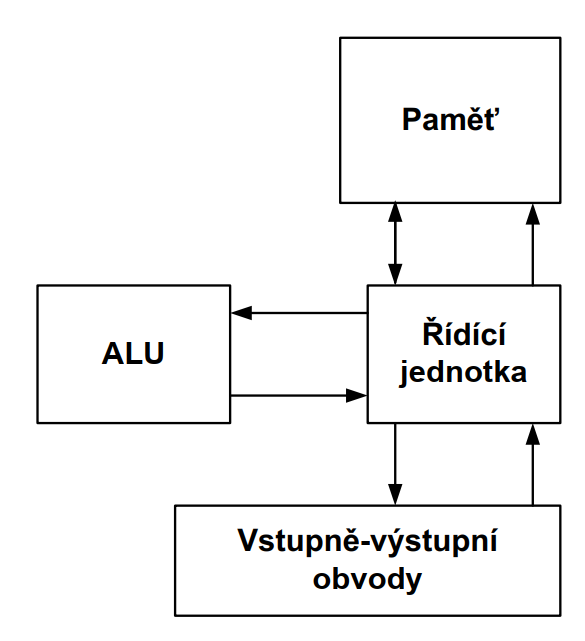
\includegraphics[scale=0.4]{images/VON.png}
   \end{center}
   \caption{Von Neumannova architektura}
  \end{figure}
  
\subsubsection{Harvardská architektura}
Chronologicky navazuje na architekturu von Neumnannovu a odstraňuje některé její nedostatky\\
Zásadní rozdíl je v oddělení paměti dat a programu\\
Program nemůže přepsat sám sebe\\
Využití pamětí realizovaných jinými technologiemi (EEPROM, Flash, FRAM, DRAM)\\
Dvě sběrnice (adresová a datová) umožňuje současný přístup k instrukcím i datům
Sekvenční vykonávání instrukcí je zachována\\
    \begin{figure}[h]
   \begin{center}
     \includegraphics[scale=0.5]{images/HAR.png}
   \end{center}
   \caption{Harvardská architektura}
  \end{figure}


\subsection{CISC}
Slovo CISC je zkráceno jako ''Complex Instruction Set Computer''. Jedná se o takovou konstrukci procesoru, která vykonává úlohu pouze pomocí jediného příkazu. Příkaz obsahuje vícekrokové operace, které chce program provést. Kromě toho mají stroje CISC relativně menší programy.

Zatímco počet složených instrukcí má obrovskou velikost. Proto vyžaduje spoustu času při provádění. V tomto typu architektury je každá sada instrukcí velmi dobře chráněna v různých krocích. To znamená, že s každou sadou instrukcí souvisí navíc tři sta instrukcí. Z tohoto důvodu trvá provádění instrukcí dlouho. Jejich doba se může pohybovat od dvou do deseti strojových cyklů v závislosti na velikosti instrukční sady. Architektura CISC navíc běžně neimplementuje pipelining, protože je to obtížné.

\textbf{Charakteristika CISC:}\\
\begin{itemize}
\item Instrukční sada je složitá. Proto je její dekódování.
\item Instrukce jsou vzhledem ke své složitosti obvykle velké. Instrukce jsou obvykle větší než velikost jednoho slova.
\item Složené instrukce obvykle zaberou při svém provádění více času než jeden takt.
\item Počet registrů pro všeobecné účely je menší. Z tohoto důvodu provádí většinu operací v samotné paměti.
\item Režimy adresování jsou obvykle složité.
\item Datových typů je mnoho.
\end{itemize}

    \begin{figure}[h]
   \begin{center}
     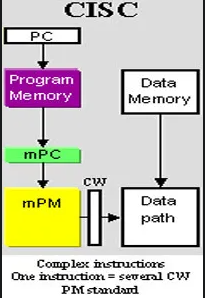
\includegraphics[scale=0.5]{images/CISC.png}
   \end{center}
   \caption{CISC}
  \end{figure}

\subsection{RISC}
Slovo RISC znamená "počítač s redukovanou instrukční sadou". Jedná se o takovou konstrukci procesoru, která se řídí jednoduchými instrukcemi a je opravdu rychlá. V podstatě se jedná o podmnožinu řady instrukcí. Zjednodušeně řečeno, každý příkaz vykonává opravdu jednoduché a malé úlohy. V takovém počítači je sada instrukcí jednoduchá a snadno implementovatelná. Proto se snadno implementují takové příkazy, které jsou opravdu složité a obtížně proveditelné jako jednotlivé instrukce. Každá instrukce má téměř stejnou délku. 

Stručně řečeno, rozděluje složité instrukce na jednoduché instrukce pomocí Pipleliningu. Pipelining je vícestupňový proces provádění instrukcí. Obvykle dokáže provést jednu instrukci v jednom strojovém cyklu.
\textbf{Charakteristika RISC:}\\
\begin{itemize}
\item Jednoduchá sada instrukcí, které se snadno dekódují a implementují.
\item Velikost jedné instrukce se vejde do velikosti jednoho slova.
\item K provedení jedné instrukce je zapotřebí pouze jeden takt, takže se jedná o rychlý proces.
\item Množství registrů pro všeobecné účely je větší.
\item Režimy adresování jsou poměrně jednoduché.
\item Proměnných datových typů je velmi málo.
\item Jeho hlavní myšlenkou je dosažení pipeliningu.
\end{itemize}
    \begin{figure}[h]
   \begin{center}
     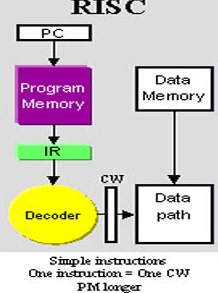
\includegraphics[scale=0.5]{images/RISC.png}
   \end{center}
   \caption{RISC}
  \end{figure}
  
\subsection{RISC vs CISC}
Široká instrukční sada procesorů CISC usnadňuje jejich
programování, protože není některé operace nutné rozepisovat (například násobení)\\
Ve strojovém kódu (nebo v jazyce symbolických adres) se dnes
programuje jen minimálně.\\
Složitost CISC procesorů vede k problémům při výrobě (velká spotřeba materiálu, větší pravděpodobnost vady, komplikovaný návrh, problémy s vysokými frekvencemi, pipelining, cache atd).\\
Typickými zástupci koncepce CISC jsou procesory rodiny Motorola 68000 a procesory postavené na architektuře Intel x86.\\

\subsection{VLIW}
VLIV (Very Long Instruction Word)\\
Efektivnější vykonávání programu\\
Podporováno hardwarové paralelní zpracování instrukcí, je realizováno větším počtem funkčních jednotek\\
Podstata paralelního zpracování:\\
Během násobení dvou čísel je možné operandy sčítat a z paměti načíst další hodnoty\\

Instrukce zpracovávány po jedné (Von Neumannově), ale:\\
Programová instrukce označena jako instrukční paket a rozdělena
do skupiny polí (dílčích instrukcí) a zde samostatně zpracována\\
Současně jsou řízeny přenosové cesty (datové i adresové)\\
Výhody: Vysoký výpočetní výkon s jednoduchou architekturou\\
    \begin{figure}[h]
   \begin{center}
     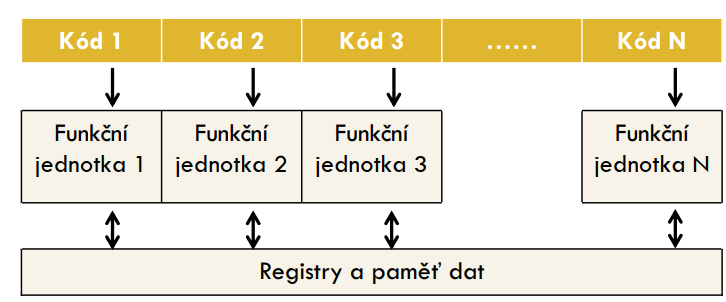
\includegraphics[scale=0.5]{images/VLIW.png}
   \end{center}
   \caption{VLIW}
  \end{figure}

\subsection{CLIW}
\subsection{ARM}
ARM ( Advanced RISC Machine) je architektura procesorů vyvinutá v Británii firmou ARM Limited\\
Nízká spotřeba energie při vysokém výpočetním výkonu\\
Schopnost práce v náročných tepelných podmínkách (nízkopříkonové procesory nepotřebují složité a relativně nespolehlivé chlazení).\\
Dnes tvoří rodina procesorů ARM 75 \% všech 32bitových RISC procesorů ve vestavěných zařízeních, což z ní dělá nejpoužívanější architekturu na světě.\\

\subsubsection{Charakteristika:}
\begin{itemize}
\item 32bitová vnitřní architektura
\item 32bitová datová sběrnice s propustností 32 MB/s
\item 26bitová adresová sběrnice (dostupný lineární adresní prostor
64 MiB)
\item 25 vnitřních 32bitových registrů
\item přístup do paměti pouze instrukcemi Load/Store
\item částečné překrývání vnitřních registrů
\item nejdelší doba reakce na přerušení 3 milisekundy
\item možnost podmíněného vykonání instrukcí
\item možnost připojení standardních pamětí DRAM
\item jednoduchý a výkonný instrukční soubor, jednoduše
využitelné kompilátory vyšších programovacích jazyků
\item Dva typy přerušení FIQ (Fast Interrupt Request)/ IRQ(Interrupt
Request)
\end{itemize}

Procesor ARM obsahuje 44 základních instrukcí s jednotnou šířkou 32 bitů.\\
V jednom taktu se vykonávají pouze instrukce pracující s aritmeticko-logickou jednotkou (ALU), s registry nebo s přímými operandy.\\
\textbf{Procesor pracuje ve čtyřech základních režimech:}
\begin{itemize}
\item uživatelský režim USR
\item privilegovaný režim supervizora SUP
\item privilegovaný režim přerušení IRQ
\item privilegovaný režim rychlého přerušení FIQ
\end{itemize}

V procesoru je obsaženo 25 částečně se překrývajících 32bitových registrů (15 registrů je univerzálních a zbývajících 10 má speciální funkce), z toho 16 registrů je v každém režimu činnosti programově přístupných.
    \begin{figure}[h]
   \begin{center}
     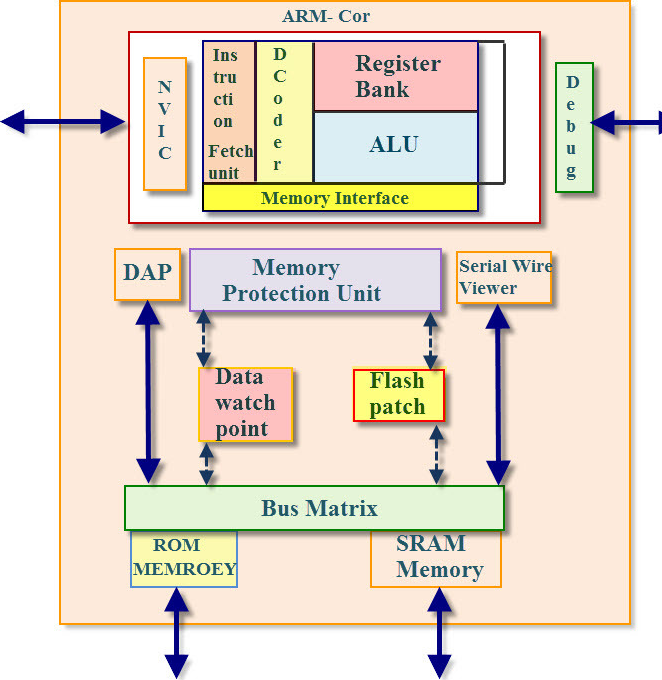
\includegraphics[scale=0.5]{images/ARM.png}
   \end{center}
   \caption{ARM}
  \end{figure}














